\section{Energy Lab}\label{sc:energylab}

To test the energy consumption of the motes, a laboratory test has been conducted on two TelosB units. on Figure \ref{fig:energyLab_testSetup} the test setup is defined. The test was conducted in the same manner as laboratory exercise 5\footnote{REF TO APPENDIX WITH LABORATORY EXERCISE 5}.

\begin{figure}[H]
	\centering
	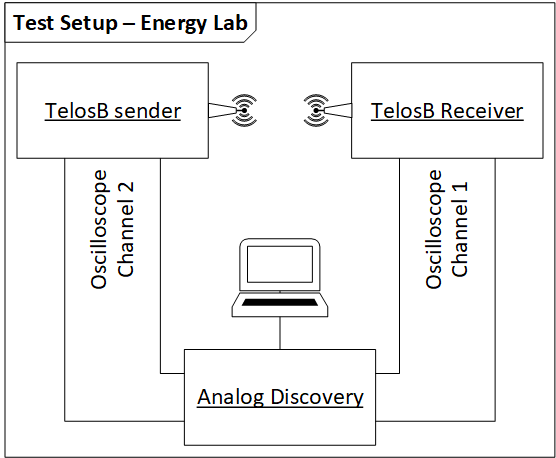
\includegraphics[width=0.8\linewidth]{implementation/energylab/fig/energyLab_testSetup.png}
	\caption{Energy lab test setup.}
	\label{fig:energyLab_testSetup}
\end{figure}

The results of the readings can be seen on Figure \ref{fig:radioOn_idle}, \ref{fig:radioOn_sendLowSignal}, \ref{fig:radioOn_sendMidSignal} and \ref{fig:radioOn_sendHighSignal}.

\begin{figure}[H]
	\centering
	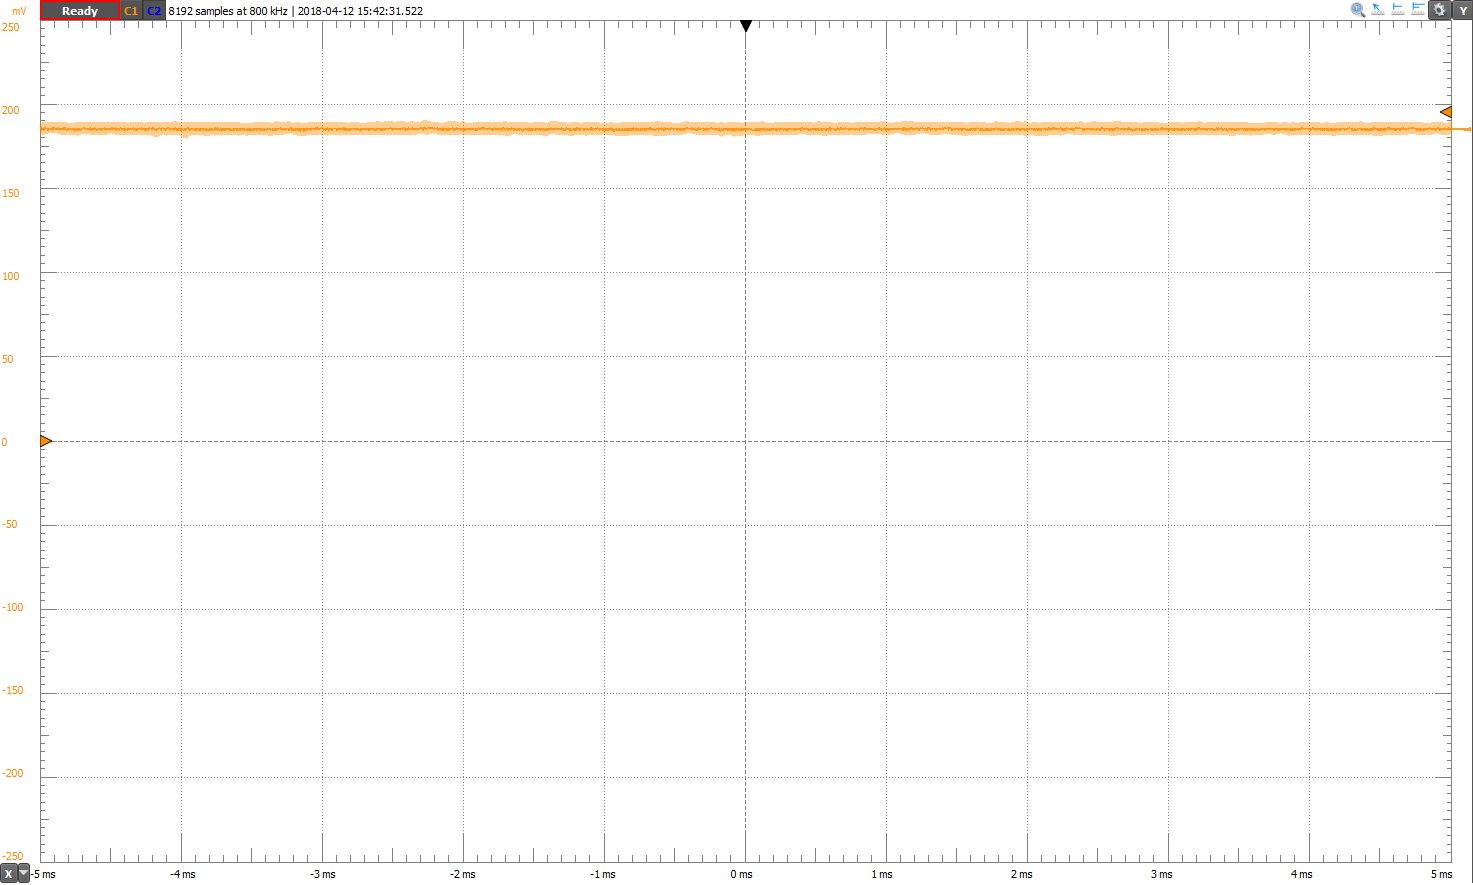
\includegraphics[width=0.8\linewidth]{implementation/energylab/fig/radioOn_idle.png}
	\caption{Voltage of Receiver (yellow), radio on, doing nothing.}
	\label{fig:radioOn_idle}
\end{figure}

\begin{figure}[H]
	\centering
	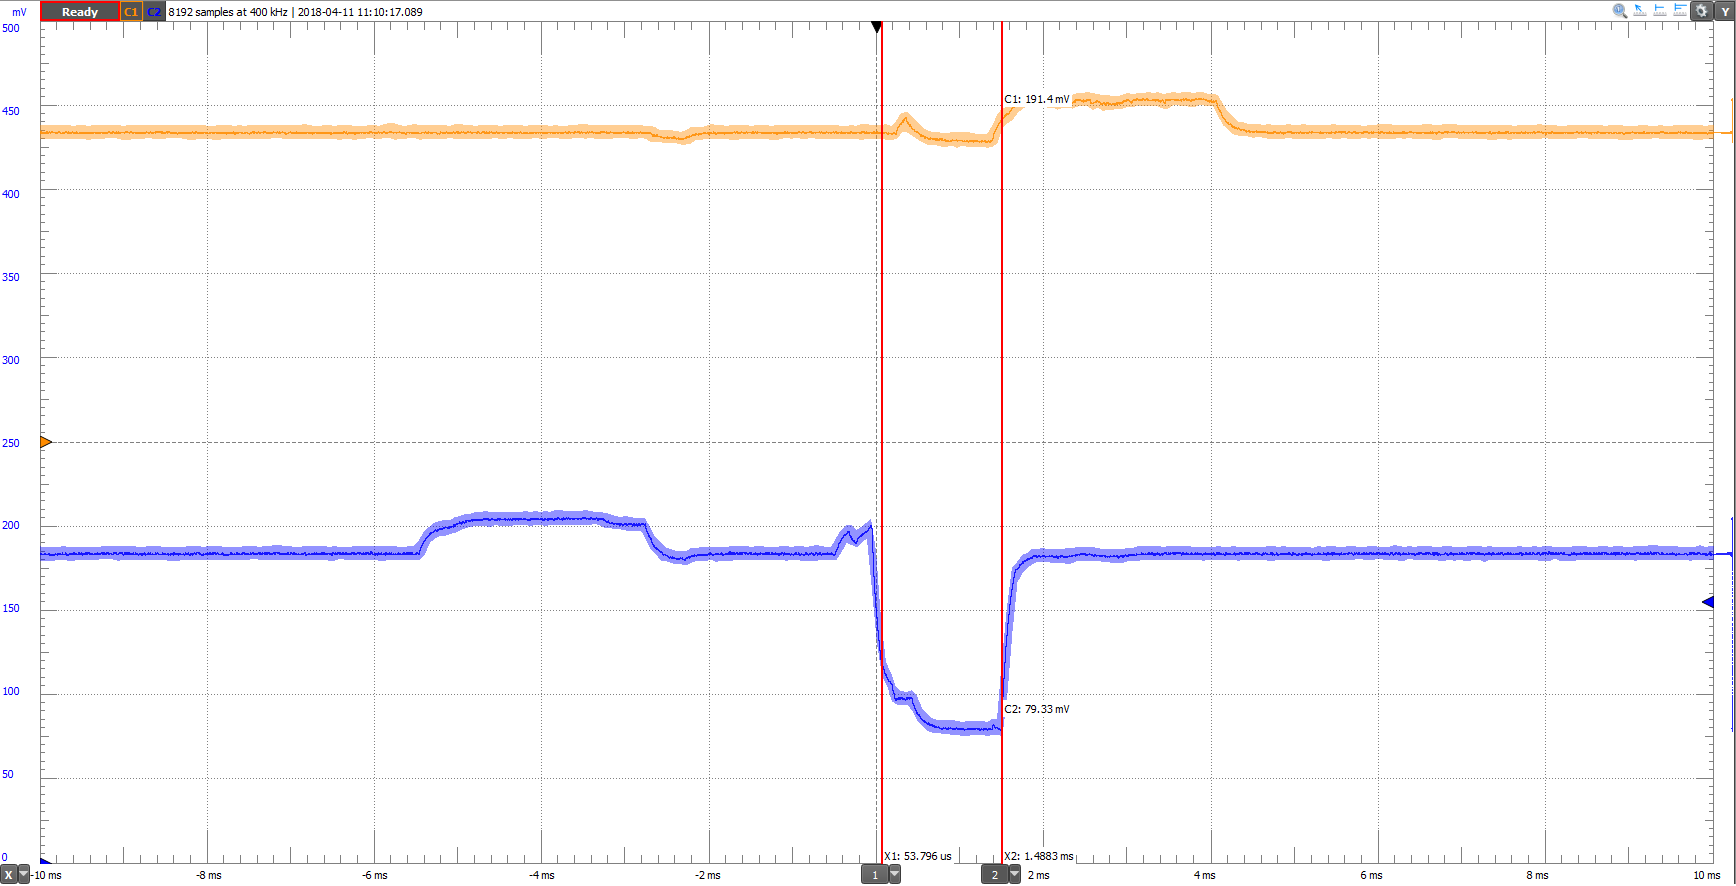
\includegraphics[width=0.8\linewidth]{implementation/energylab/fig/radioOn_sendLowSignal.png}
	\caption{Voltage of Sender (blue) and Receiver (yellow), radio on, sending at $-25.0dBm$.}
	\label{fig:radioOn_sendLowSignal}
\end{figure}

\begin{figure}[H]
	\centering
	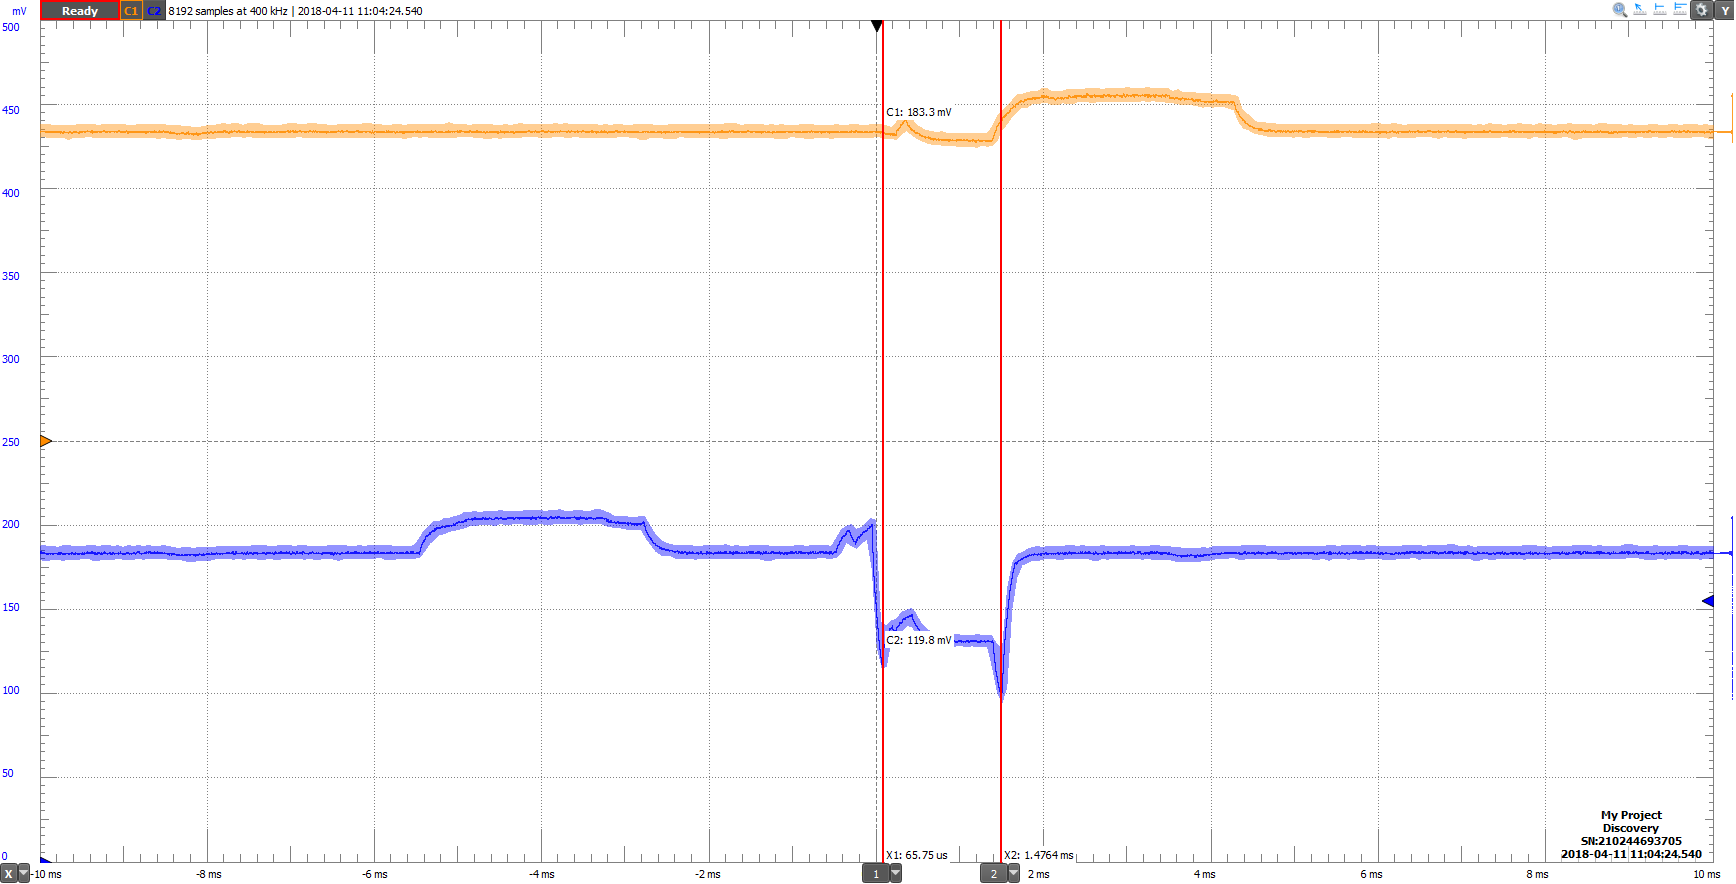
\includegraphics[width=0.8\linewidth]{implementation/energylab/fig/radioOn_sendMidSignal.png}
	\caption{Voltage of Sender (blue) and Receiver (yellow), radio on, sending at $-12.5dBm$.}
	\label{fig:radioOn_sendMidSignal}
\end{figure}

\begin{figure}[H]
	\centering
	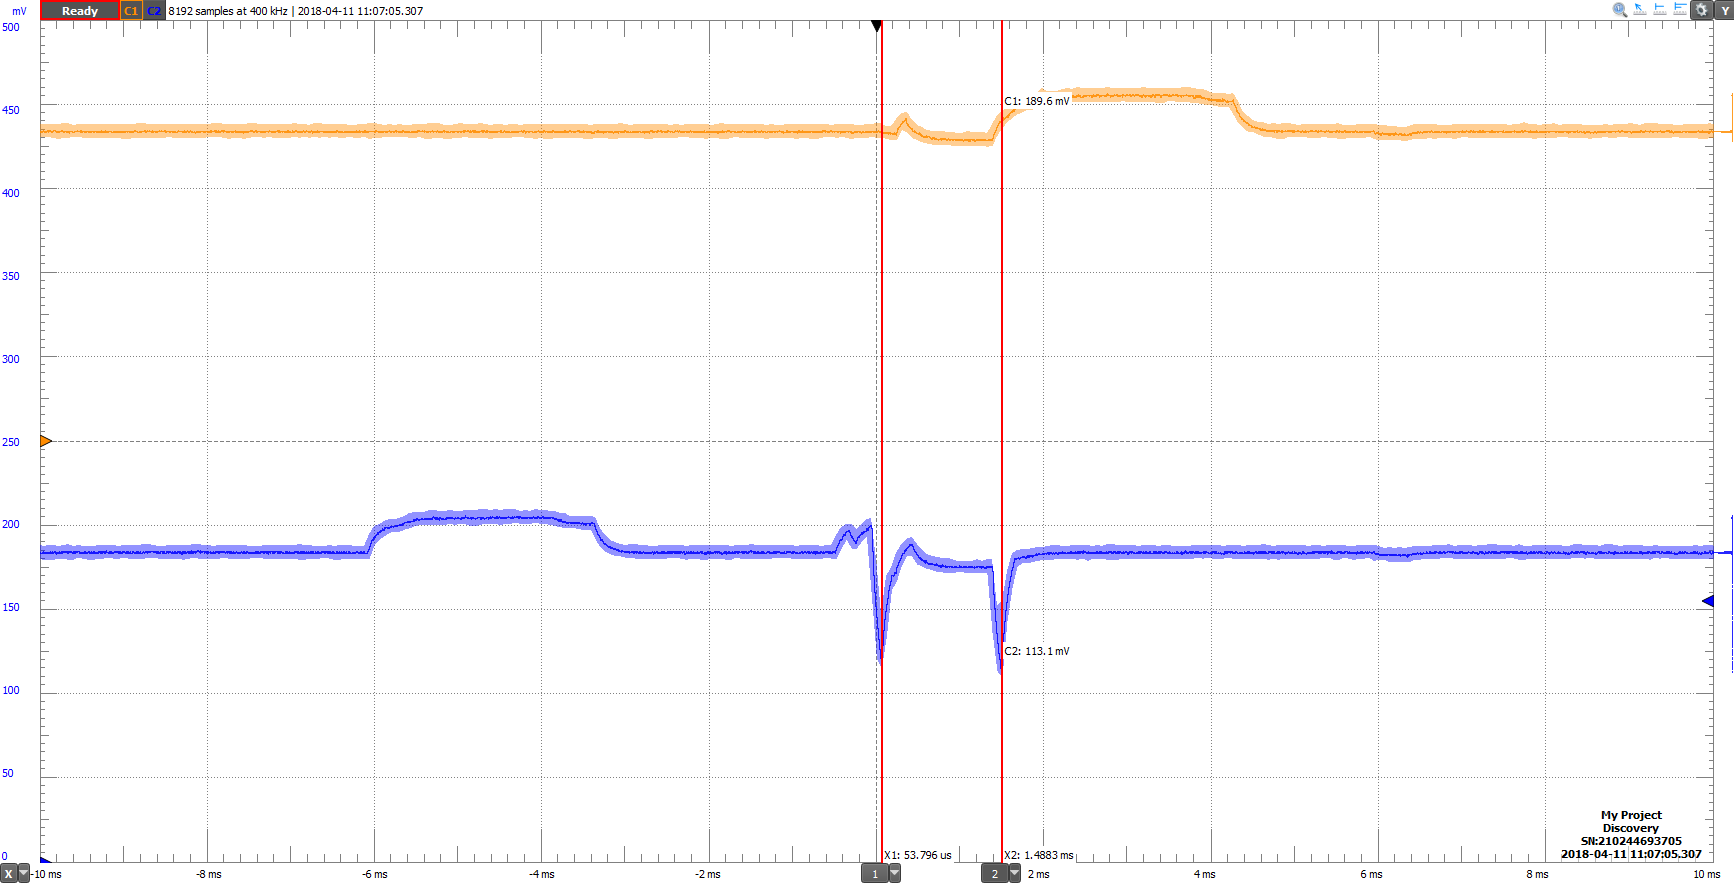
\includegraphics[width=0.8\linewidth]{implementation/energylab/fig/radioOn_sendHighSignal.png}
	\caption{Voltage of Sender (blue) and Receiver (yellow), radio on, sending at $0.0dBm$.}
	\label{fig:radioOn_sendHighSignal}
\end{figure}

